\sep
\section{Grundlagen}
\Satz[1.1] Es gibt keine Gleichung der Form  \[x^n + a_{n-1}x^{n-1}+...+a_0 = 0\]
mit \(a_i \in \Q \), so dass \(x = \pi\) eine Lösung ist \newline
\Satz[1.2] \(R\) ist ein kommutativer, angeordneter Körper, der ordnungsvollständig ist \newline
\Def[Axiome der Addition]
\begin{enumerate}
    \item [A1] Assoziativität \(x+(y+z) = (x+y)+z\)
    \item [A2] Neutrales Element \(x + 0 = x \quad \forall x \in \R\)
    \item [A3] Inverses Element \(\forall x \in \R \  \exists y \in \R: x+y=0\)
    \item [A4] Kommutativität \(x + z = z + x \quad \forall x,z \in \R \)
\end{enumerate}
\Def[Axiome der Multiplikation]
\begin{enumerate}
    \item[M1] Assoziativität \(x \cdot (y \cdot z) = (x \cdot y) \cdot z \quad \forall x,y,z \in R\)
    \item[M2] Neutrales Element \(x \cdot 1 = x \quad \forall x \in \R \)
    \item[M3] Inverses Element \( \forall x \in \R, x \neq 0 \ \exists y \in \R : \newline x \cdot y = 1\)
    \item[M4] Kommutativität \( x \cdot z = z \cdot x \quad \forall x,z \in \R \)
\end{enumerate}
\Def[Distributivität]
\begin{enumerate}
    \item [D1] Distributivität \(x \cdot (y + z) = x \cdot y + x \cdot z\)
\end{enumerate}
\Def[Ordnungsaxiome]
\begin{enumerate}
    \item[O1] Reflexivität  \(x \leq x  \quad \forall x \in \R \)
    \item[O2] Transitivität \(x \leq y\) and \(y \leq z \implies x \leq z\)
    \item[O3] Antisymmetrie \(x \leq y\) and \(y \leq x \implies x = y\)
    \item[O4] Total \(\forall x,y \in \R\) gilt entweder \(x \leq y$ oder $y \leq x \)
\end{enumerate}
\Def[Kompatibilität]
\begin{enumerate}
    \item[K1] \(\forall x,y,z \in \R: x \leq y \implies x + z \leq y + z \)
    \item[K2] \(\forall x \geq 0, \forall y \geq 0: x \cdot y \geq 0\)
\end{enumerate}
\Def[Ordnungsvollständigkeit] \newline 
Seien A,B \(\subseteq\) von \(\R\)
\begin{enumerate}
    \item [i] \(A \neq \emptyset, B \neq \emptyset\)
    \item [ii] \(\forall a \in A$ and $\forall b \in B: a \leq b\)
\end{enumerate}
Dann gibt es \(c \in \R\), dass \(\forall \in A : a \leq c\) und \(\forall b \in B: c \leq b\) \newline
\includegraphics[scale=0.500]{Ordnungsvollständigkeit.png}
\Korollar[1.6]
\begin{enumerate}
    \item [1] Additive und multiplikate Inverse eindeutig
    \item [2] \(0 \cdot x = 0 \quad \forall x \in \R \)
    \item [3] \((-1) \cdot x = -x \quad \forall x \in \R \)
    \item [4] \(y \geq 0 \Leftrightarrow (-y) \leq 0\)
    \item [5] \(y^2 \geq 0 \quad \forall x \in \R \)
    \item [6] \(x \leq y $ and $u \leq v \implies x+ u \leq y + v\)
    \item [7] \(0 \leq x \leq y\) und \(0 \leq u \leq v \implies x \cdot u \leq y \cdot v\)
    \newline \newline
\end{enumerate}

\Korollar[1.7(Archimedisches Prinzip)] \newline
Sei \(x \in \R\) mit \(x > 0\) und \(y \in \R\).Dann gibt es \(n \in \N\) mit \(y \leq n \cdot x\) \newline \newline \newline
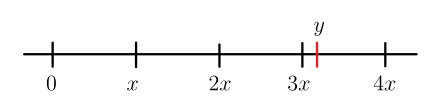
\includegraphics[scale=0.400]{Archimedisches_Prinzip.png}
\Satz[1.8] \newline
Für jedes \(t \geq 0, t \in \R\) hat \(x^2 = t\) eine Lösung in \(\R\) \newline
\Def[1.9] Seien \(x,y \in \R \) \newline
\begin{enumerate}
    \item [(i)] max\{x,y\} \(= \left\{\begin{array}{lll}
        x & \text { falls } & y \leq x \\
        y & \text { falls } & x \leq y
        \end{array}\right.\)
    \item[(ii)] min\{x,y\}  \(= \left\{\begin{array}{lll}
        y & \text { falls } & y \leq x \\
        x & \text { falls } & x \leq y
        \end{array}\right.\)
    \item[(iii)]  Der Absolutbetrag einer Zahl \(x \in \R: \newline \abs{x} = max\{x, -x\}\)
\end{enumerate}
\Satz[1.10]
\begin{enumerate}
    \item [(i)] \( \abs{x} \geq 0 \quad \forall x \in \R \)
    \item [(ii)] \(\abs{xy} = \abs{x}\abs{y} \quad \forall x,y \in \R \)
    \item [(iii)] \(\abs{x+ y} \leq \abs{x} + \abs{y} \quad \forall x,y \in \R\)
    \item [(iv)] \( \abs{x + y} \geq \abs{x} - \abs{y} \quad \forall x,y \in \R\)
\end{enumerate}
\Satz[1.11(Young'sche Ungleichung)] \newline
\(\forall \epsilon > 0, \forall x,y \in \R \):
\[2 \abs{xy} \leq \epsilon x^2 + \frac{1}{\epsilon}y^2\]
\sep
\subsection{Infimum und Supremum}
\Def[1.12]  Sei \(A \subseteq \R\) eine Teilmenge.
\begin{enumerate}
\item[1)]  \(c \in \R\) ist \textbf{obere Schranke} if  \(\forall a \in A: a \leq c\)
\item[2)]  \(c \in \R\) ist \textbf{untere Schranke} if \(\forall a \in A: c \leq a\)
\item[3)] \(m \in \R\) heisst ein \textbf{Maximum} von A if \(m \in A\) und \(m\) eine obere Schranke von A ist.
\item[4)] \(m \in \R\) heisst ein \textbf{Minimum} von A if \(m \in A\) und \(m\) eine untere Schranke von A ist.
\end{enumerate}

\Satz[1.15]. Sei \(A \subseteq \R, A \neq \emptyset\)
\begin{enumerate}
\item[1)]  Sei A nach oben beschränkt. Dann gibt es eine kleinste obere Schranke: 
\[c:=\sup A \text{ \ \textbf{(Supremum von A)}}\]
\item[2)]  Sei A nach unten beschränkt. Dann gibt es eine grösste untere Schranke: 
\[d:=\inf A \text{ \ \textbf{(Infimum von A)}} \]  
\end{enumerate}

Eigenschaften von Supremum und Infimum
\begin{enumerate}
\item[\(\bullet\)]  \(\sup (A \cup B) = \text{max} (\sup A, \sup B)\)
\item[\(\bullet\)]  \(\sup (A + B) = \sup A + \sup B\)
\item[\(\bullet\)]  \(\inf (A \cup B) = \text{min} (\inf A, \inf B)\)
\item[\(\bullet\)]  \(\inf (A + B) = \inf A + \inf B\)
\end{enumerate}
\Korollar[1.16]  Seien \(A \subseteq B \subseteq \R\) Teilmengen von \(\R\)
\begin{enumerate}
    \item [1] Falls B nach oben beschränkt ist, \newline \(\sup A \leq \sup B\)
    \item [2] Falls B nach unten beschränkt ist, \newline\(\inf B \leq \inf A\)
\end{enumerate}
\sep
\Def[1.18] Kardinalität
\begin{enumerate}
    \item [(i)] Zwei Mengen X,Y heissen gleichmächtig if eine Bijection \(f: X \rightarrow Y\) existiert
    \item [(ii)] Eine Menge ist endlich, wenn \(X = \emptyset\) or \(\exists n \in \N\) so dass\(\{1,2,\dots,n\}\)gleichmächtig wie X
    \item [(iii)] Eine Menge X ist abzähbar if endlich oder gleichmächtig wie \(\N\)
\end{enumerate}
\Satz[1.20] (Cantor) \(\R\) ist nicht abzählbar
